\documentclass[landscape,a0paper,fontscale=0.292]{baposter}
\usepackage[vlined]{algorithm2e}
\usepackage{times}
\usepackage{calc}
\usepackage{url}
\usepackage{graphicx}
\usepackage{amsmath}
\usepackage{amssymb}
\usepackage{relsize}
\usepackage{multirow}
\usepackage{booktabs}
\usepackage{multicol}
\usepackage[T1]{fontenc}
	\usepackage{ae}
 \usepackage{setspace}

\usepackage{enumitem} % to reduce identation in itemize, etc

% One-lien spacing in bibliography
  \let\oldthebibliography=\thebibliography
  \let\endoldthebibliography=\endthebibliography
  \renewenvironment{thebibliography}[1]{%
    \begin{oldthebibliography}{#1}%
      \setlength{\parskip}{0ex}%
      \setlength{\itemsep}{0ex}%
  }%
  {%
    \end{oldthebibliography}%
  }



\definecolor{lightgreen}{rgb}{0,1,0}
\definecolor{lightblue}{rgb}{0.2,0.2,1}
\newcommand{\Green}[1]{\color{lightgreen}{#1}\color{black}}
\newcommand{\Blue}[1]{\color{lightblue}{#1}\color{black}}
\newcommand{\structure}[1]{{\color{blue}{#1}}}
\newcommand{\red}[1]{{\color{red}#1}}

% My commands here
\DeclareMathAlphabet{\mathpzc}{OT1}{pzc}{m}{it}
\newcommand{\insertline}{\vspace{2mm}}

% genereal purpose macros here
\newcommand{\marg}{\marginpar}
\newcommand{\todo}[1]{{\color{red}{TODO: #1}}}
\newcommand{\commentOut}[1]{} 
\newcommand{\add}[1]{\textcolor{red}{#1}} % To highligh modified text

% abbreviations
\newcommand{\etal}{et al.\xspace}
\newcommand{\ie}{i.e.\xspace}
\newcommand{\eg}{e.g.\xspace}
\newcommand{\Ie}{I.e.\xspace}



% Matrices and vectors 
\newcommand{\mat}[1]{\mathbf{#1}}
\renewcommand{\vec}[1]{ \mathbf{#1} } % math bold
\newcommand{\vecS}[1]{\boldsymbol{ #1 }  } % this for boldsymbols
\newcommand{\vecentry}[2]{{\mathrm #1_{#2}}}
\newcommand{\matentry}[3]{{\mathrm #1_{#2,#3}}}
\newcommand{\matcol}[2]{\mat{#1}_{\cdot #2}}
\newcommand{\matrow}[2]{\mat{#1}_{#2 \cdot}}

 % Matrices here
 \newcommand{\A}{\mat{A}}
\newcommand{\B}{\mat{B}}
\newcommand{\C}{\mat{C}}
\newcommand{\D}{\mat{D}}
\newcommand{\F}{\mat{F}}
\newcommand{\G}{\mat{G}}
\newcommand{\I}{\mat{I}}
\renewcommand{\L}{\mat{L}}
\newcommand{\X}{\mat{X}}
\newcommand{\W}{\mat{W}}
\newcommand{\Y}{\mat{Y}}
\newcommand{\Z}{\mat{Z}}
\renewcommand{\S}{\mat{S}}
\newcommand{\K}{\mat{K}}
\newcommand{\U}{\mat{U}}

% Vectors here
\newcommand{\f}{\vec{f}}
\newcommand{\g}{\vec{g}}
\newcommand{\h}{\vec{h}}
\newcommand{\m}{\vec{m}}
\renewcommand{\t}{\vec{t}}
\renewcommand{\u}{\vec{u}}
\renewcommand{\v}{\vec{v}}
\newcommand{\w}{\vec{w}}
\newcommand{\x}{\vec{x}}
\newcommand{\y}{\vec{y}}
\newcommand{\z}{\vec{z}}
\newcommand{\s}{\vec{s}}

 % Vectorial greek letters
  \newcommand{\vecmu}{\vecS{\mu}}
 \newcommand{\vectheta}{\vecS{\theta}}
 \newcommand{\vecalpha}{\vecS{\alpha}}
 \newcommand{\vecphi}{\vecS{\phi}}
 \newcommand{\veceta}{\vecS{\eta}}
 \newcommand{\vecepsilon}{\vecS{\epsilon}} 
 
% caligraphic alphabet
\newcommand{\calA}{\mathcal{A}}
\newcommand{\calC}{\mathcal{C}}
\newcommand{\calD}{\mathcal{D}} 
\newcommand{\calL}{\mathcal{L}}
\newcommand{\calM}{\mathcal{M}}
\newcommand{\calT}{\mathcal{T}}
\newcommand{\calU}{\mathcal{U}}
\newcommand{\calX}{\mathcal{X}}
\newcommand{\calF}{\mathcal{F}}
\newcommand{\calE}{\mathcal{E}}
\newcommand{\calH}{\mathcal{H}}
\newcommand{\calI}{\mathcal{I}}
\newcommand{\calS}{\mathcal{S}}
\newcommand{\calY}{\mathcal{Y}}
\newcommand{\calO}{\mathcal{O}}
\newcommand{\calQ}{\mathcal{Q}}
\newcommand{\calR}{\mathcal{R}}
\newcommand{\calV}{\mathcal{V}}


% blackboard alphabet 
\newcommand{\setR}{\mathbb{R}}
\newcommand{\setE}{\mathbb{E}}
\newcommand{\setV}{\mathbb{V}}
\newcommand{\setI}{\mathbb{I}}
\newcommand{\setX}{\mathbb{X}}
\newcommand{\setT}{\mathbb{T}}



% Useful math operators
\newcommand{\Sum}{{\displaystyle \sum}}
\DeclareMathOperator{\vect}{vec}
\DeclareMathOperator{\diag}{diag}
\DeclareMathOperator*{\argmax}{argmax}                 
\DeclareMathOperator*{\argmin}{argmin}                 
\providecommand{\abs}[1]{\lvert#1\rvert}
\providecommand{\norm}[1]{\lVert#1\rVert}
\newcommand{\notp}[1]{\stackrel{\neg}{#1}} % symbol for not present


% matrix products
\newcommand{\kron}{\otimes}
\newcommand{\hada}{\bullet}

% statistics
\newcommand{\expectation}{\mathbb{E}}
\newcommand{\Eb}[1]{\left\langle #1 \right\rangle} % Expectation in angle brackets
\newcommand{\variance}{\mathbb{V}}
\newcommand{\Normal}{\mathcal{N}}  
\newcommand{\avg}[1]{\overline{#1}}
\newcommand{\KL}{\text{KL}}

% GP things
\newcommand{\GP}{\mathcal{GP}}
\newcommand{\kernel}{\kappa}

% Other maths
\newcommand{\deriv}[2]{\frac{\partial{#1}}{\partial{#2}}}
\newcommand{\trace}{\mbox{ \rm tr }}
\renewcommand{\det}[1]{\lvert#1\rvert}
\newcommand{\defeq}{\stackrel{\text{\tiny def}}{=}}
\newcommand{\idx}{\mathcal{I}}
\newcommand{\T}{\text{T}}
\newcommand{\mth}{\mathrm{th}} 


\newcommand{\bigO}{\calO}
\newcommand{\define}{\overset{\Delta}{=}}




















\newcommand{\entropy}{\calH}

\newcommand{\sigmak}{\sigma_{k}}
\newcommand{\der}{\mathrm{d}}

\newcommand{\sigmanoise}{\sigma_{\text{n}}}
\newcommand{\sigmoid}{\text{sig}}
\newcommand{\bs}{\boldsymbol}
\newcommand{\xstar}{x_*}
\newcommand{\fstar}{f_*}
\newcommand{\ystar}{y_*}
\newcommand{\zstar}{z_*}
\newcommand{\vxstar}{\x_*}
\newcommand{\vfstar}{\f_*}

% automated variational inference for gps
\newcommand{\llambda}{\bs{\lambda}}
%\newcommand{\fn}{\f_{(n)}}
\newcommand{\vtheta}[1]{\bs{\theta}_{#1}}
\newcommand{\Ljoint}{\calL_{\text{joint}}}
\newcommand{\Lent}{\calL_{\text{ent}}}
\newcommand{\Lcross}{\calL_{\text{cross}}}
\newcommand{\vystar}{\y_{*}}
\newcommand{\Ystar}{\Y_{*}}

%
\newcommand{\fj}{\f_{\hada j}}
\newcommand{\fn}{\f_{n \hada}}

% methods
\newcommand{\agp}{{\sc{AGP}}}
\newcommand{\agpfull}{{\sc{AGP-FULL}}}
\newcommand{\agpmix}{{\sc{AGP-MIX}}}
\newcommand{\agpmixtwo}{{\sc{AGP-MIX2}}}
\newcommand{\gpr}{{\sc{GPR}}}
\newcommand{\wgp}{{\sc{WGP}}}
\newcommand{\ep}{{\sc{EP}}}
\newcommand{\vb}{{\sc{VB}}}
\newcommand{\vq}{{\sc{VQ}}}
\newcommand{\vbo}{{\sc{VBO}}}
\newcommand{\hmc}{{\sc{HMC}}}
\newcommand{\ess}{{\sc{ESS}}}
\newcommand{\full}{{\sc{FULL}}}
\newcommand{\mix}{{\sc{MIX}}}
\newcommand{\mixtwo}{{\sc{MIX2}}}





 %%%%%%%%%%%%%%%%%%%%%%%%%%%%%%%
 % Save space in lists. Use this after the opening of the list
 %%%%%%%%%%%%%%%%%%%%%%%%%%%%%%%
 \newcommand{\compresslist}{%
 \setlength{\itemsep}{1pt}%
 \setlength{\parskip}{0pt}%
 \setlength{\parsep}{0pt}%
 }


 %%%%%%%%%%%%%%%%%%%%%%%%%%%%%%%
 % Multicol Settings
 %%%%%%%%%%%%%%%%%%%%%%%%%%%%%%%
 \setlength{\columnsep}{0.7em}
 \setlength{\columnseprule}{0mm}


\graphicspath{{./figures/}}



%%%%%%%%%%%%%%%%%%%%%%%%%%%%%
%% Begin of Document
%%%%%%%%%%%%%%%%%%%%%%%%%%%%%
\begin{document}
%%%%%%%%%%%%%%%%%%%%%%%%%%%%%
%% Here starts the poster
%%---------------------------------------------------------------------------
%% Format it to your taste with the options
%%%%%%%%%%%%%%%%%%%%%%%%%%%%%
\begin{poster}{
 % Show grid to help with alignment
 grid=false,
 columns=3,
 % Column spacing
 colspacing=0.7em,
 % Color style
 headerColorOne=cyan!20!white!90!black,
 borderColor=cyan!30!white!90!black,
 % Format of textbox
%textborder=faded,
textborder=rounded,
 % Format of text header
 headerborder=open,
 headershape=roundedright,
 headershade=plain,
 background=none,
%bgColorOne=cyan!10!white,
  bgColorOne=white,
  bgColorTwo=white,
  boxColorOne=white,
 headerheight=0.12\textheight}
 % Eye Catcher
 {
     % \includegraphics[width=0.08\linewidth]{track_frame_00010_06}
 }
 % Title % FIXME: INSERT POSTER NUMBER
 {
 \sc  
	Automated Variational Inference for Gaussian Process Models
 }
  % Authors
  { 
   \vspace{5mm} 
   \smaller{ 
   \begin{tabular}{cc}
     Trung V. Nguyen &  Edwin V. Bonilla \\
      {\texttt{VanTrung.Nguyen@nicta.com.au}} &  { \texttt{e.bonilla@unsw.edu.au} } \\
     	ANU \& NICTA	&       The University of New South Wales
    \end{tabular}
   }   
 }
 %
 % University logo
 {
   \begin{tabular}{c}
   \centering
      
\includegraphics[height=0.1\textheight]{logo-nicta} \hspace{5mm}
     
\includegraphics[height=0.1\textheight]{logo-unsw}
   \end{tabular}
 }


%%%%%%%%%%%%%%%%%%%%%%%%%%%%%%%%%%%%%%%%%%%%%%%%%%%%%%%%%%%%%%%%%%%%%%%%%%%%%%
%%% Now define the boxes that make up the poster
%%%---------------------------------------------------------------------------
%%% Each box has a name and can be placed absolutely or relatively.
%%% The only inconvenience is that you can only specify a relative position 
%%% towards an already declared box. So if you have a box attached to the 
%%% bottom, one to the top and a third one which should be inbetween, you 
%%% have to specify the top and bottom boxes before you specify the middle 
%%% box.
%%%%%%%%%%%%%%%%%%%%%%%%%%%%%%%%%%%%%%%%%%%%%%%%%%%%%%%%%%%%%%%%%%%%%%%%%%%%%%

%---------------------------------------------------------------
% Abstract
%---------------------------------------------------------------

 \headerbox{Bayesian Inference}{name=motivation,column=0,row=0,span=1}{ 
%
\textbf{Main problem:}  Trade-off flexibility $\leftrightarrow$ efficiency:
\begin{itemize}[leftmargin=0.5cm]
 \compresslist
\item 
\structure{Stochastic:} MCMC $\rightarrow$ flexible but high computational cost 
and cumbersome convergence analysis.
\item
\structure{Deterministic:} Variational, EP, Laplace $\rightarrow$  fast but derivations 
are model-specific. 
\end{itemize}
\textbf{Our  goal:} \emph{Build highly automated and efficient inference methods.}
\begin{itemize}[leftmargin=0.5cm]
\item
 \compresslist
	We focus  on Gaussian process (GP) priors and variational inference.
\end{itemize}
}
 

%---------------------------------------------------------------
% 
%---------------------------------------------------------------

\headerbox{Our Approach at a Glance}{name=approach,column=0,below=motivation}{
%
\begin{center}
	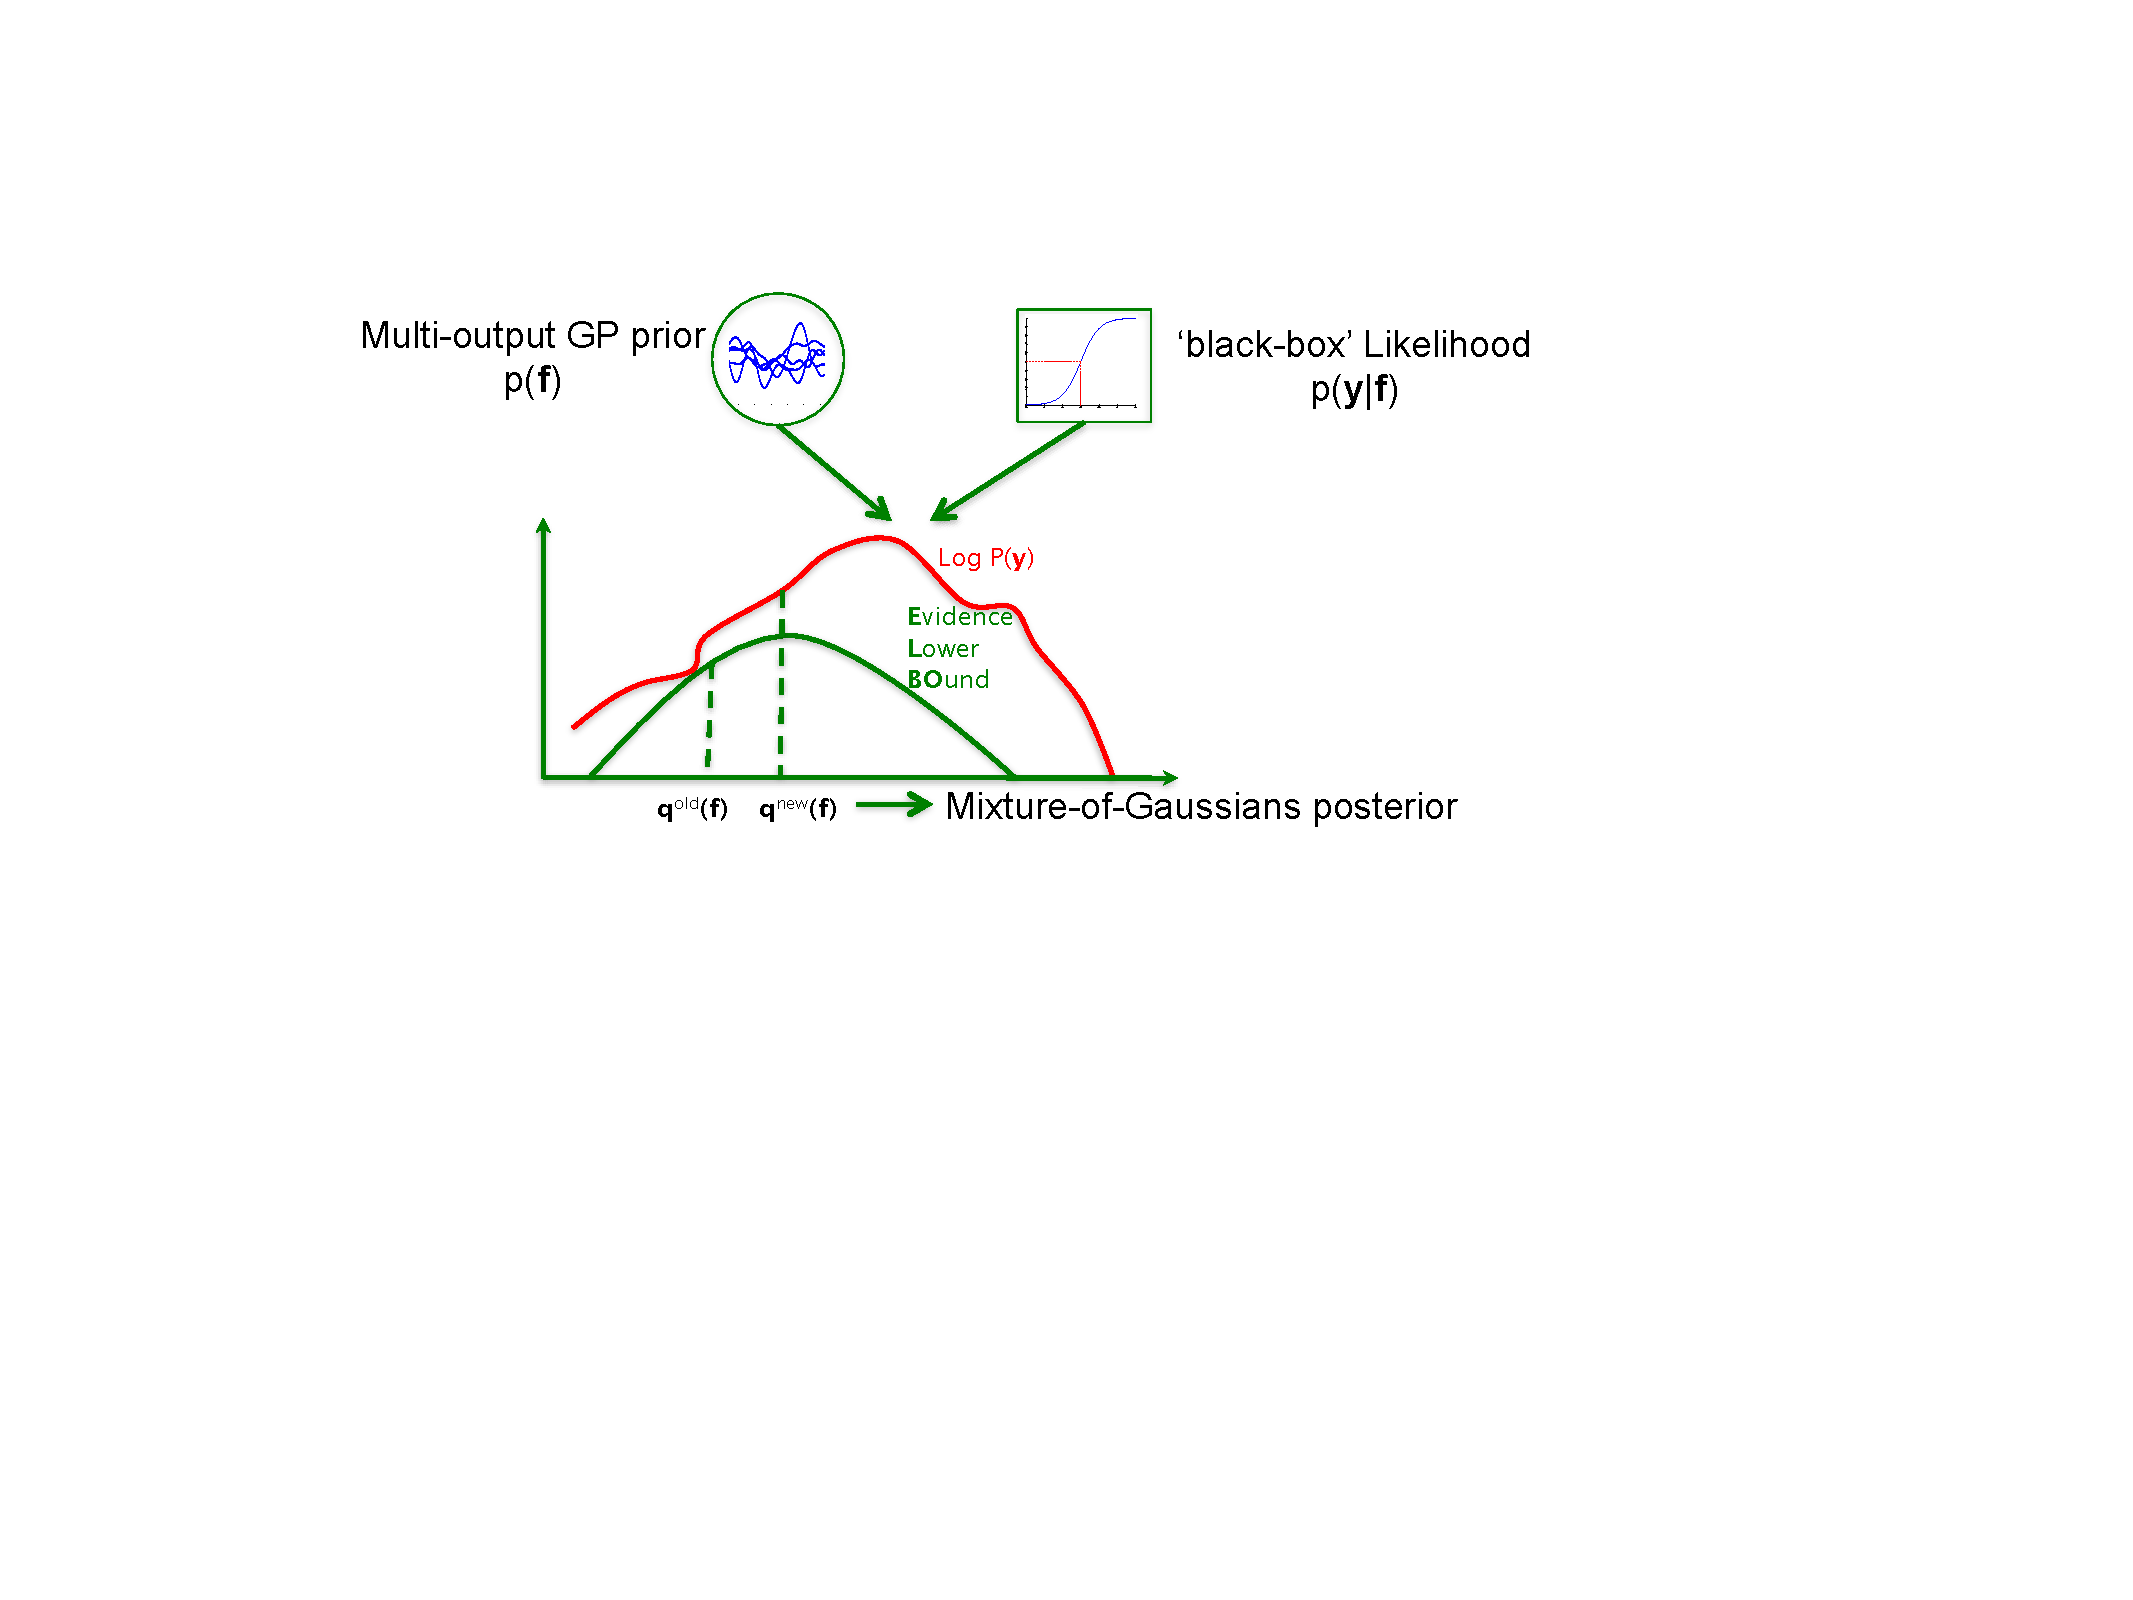
\includegraphics[width=0.8\textwidth]{avinewpdf}
\end{center}
\vspace{-0.5cm}
\textbf{Key results:}
\begin{enumerate}[leftmargin=0.5cm]
 \compresslist
\item
	Variational objective (ELBO) and its gradients are approximated efficiently: 
	expectations over \emph{univariate} Gaussians.
\item
	Efficient parameterisation of posterior covariances.
\item	
	As good as hand-coded solutions and 
%\item
	orders of magnitude faster than MCMC.
\end{enumerate}
}

%---------------------------------------------------------------
% 
%---------------------------------------------------------------

\headerbox{Latent Gaussian Process Models}{name=setting,column=0,below=approach}{
\textbf{Supervised learning problems:} $\x = \{\x_n\}_{n=1}^N$, $\y = \{\y_n\}_{n=1}^N$

\insertline
\textbf{Factorisation of GP prior over Q latent functions:}
\begin{equation}
f_j \sim \GP(0, \kernel_j(\cdot, \cdot))
\rightarrow p(\f | \vtheta{0}) = \prod_{j=1}^Q p(\fj | \vtheta{0}) = \prod_{j=1}^Q \Normal(\fj; \vec{0}, \K_j) 
\end{equation}
%\kernel_j

\insertline
\textbf{Factorisation of conditional likelihood across observations:}
\begin{equation}
p(\y | \f, \vtheta{1}) = \prod_{n=1}^N p(\y_n | \fn, \vtheta{1}) 
\end{equation}
}

%---------------------------------------------------------------
% The Model
%---------------------------------------------------------------

\headerbox{Automated  Inference Framework}{name=framework,column=1}{
\begin{equation}
\calL =  \underbrace{\expectation_q [ - \log q(\f | \llambda)] + \expectation_q  [\log p(\f)]}_{-\KL[q(\f | \llambda) || p(\f)]} +\underbrace{\sum_{k=1}^K \pi_k \expectation_{q_k}  [\log p(\y | \f)]}_{\text{ELL}}
\end{equation}
}

%---------------------------------------------------------------
% Bag of features
%---------------------------------------------------------------
\headerbox{Expected Log Likelihood Term}{name=ellterm,column=1,below=framework}{
}
\headerbox{KL Divergence Term}{name=klterm,column=1,below=ellterm}{
}





%---------------------------------------------------------------
% Results
%---------------------------------------------------------------

\headerbox{Practical Variational Distributions}{name=practical,column=1,below=klterm}{
}



%---------------------------------------------------------------
% Experiments
%---------------------------------------------------------------

\headerbox{Experiments \& Results}{name=experiments,column=2}{

}



  

%
\headerbox{References}{name=bibliography,column=1, below=practical,span=2}{
{%\tiny
\renewcommand{\refname}{\vspace{-0.9em}}
\bibliographystyle{unsrt}
\bibliography{references,mlreferences}
%\end{spacing}
}
}


\end{poster}

\end{document}
